\documentclass[11pt, oneside]{article}   	% use "amsart" instead of "article" for AMSLaTeX format
\usepackage{geometry}                		% See geometry.pdf to learn the layout options. There are lots.
\geometry{letterpaper}                   		% ... or a4paper or a5paper or ... 
%\geometry{landscape}                		% Activate for rotated page geometry
%\usepackage[parfill]{parskip}    		% Activate to begin paragraphs with an empty line rather than an indent
\usepackage{graphicx}				% Use pdf, png, jpg, or eps§ with pdflatex; use eps in DVI mode
								% TeX will automatically convert eps --> pdf in pdflatex		
\usepackage{amssymb}
\usepackage{mathrsfs}

%% some handy things for making bold math
\def\bm#1{\mathpalette\bmstyle{#1}}
\def\bmstyle#1#2{\mbox{\boldmath$#1#2$}}
\newcommand{\thh}{^\mathrm{th}}

\newcommand{\PHS}{\mathrm{PHS}}
\newcommand{\MHS}{\mathrm{MHS}}
\newcommand{\HS}{\mathrm{HS}}
\newcommand{\FS}{\mathrm{FS}}
\newcommand{\Un}{\mathrm{Un}}
\newcommand{\bT}{\mathbf{\Theta}}
\newcommand{\bM}{\bm{M}}
\newcommand{\bH}{\bm{H}}
\newcommand{\bY}{\bm{Y}}
\newcommand{\bz}{\bm{z}}
\newcommand{\BY}{\mathbf{Y}}
\newcommand{\BP}{\mathbf{P}}
\newcommand{\BPhi}{\mathbf{\Phi}}

\title{An Acyclic Directed Graph Perspective on CKMR}
\author{Eric C. Anderson}
%\date{}							% Activate to display a given date or no date

\begin{document}
\maketitle

\section{Introduction}

Reading over the recent paper on bioRxiv about {\em Glyphis} sharks, I felt like it would be good for me to
step back and think a little more generally about how these models are constructed, and what the likelihood
looks like as a directed graphical model.  I felt this way, because doing so always helps to remind me about
what is required in inference, and I think it could make the {\em Glyphis} paper a little more clear.  The authors
of that paper describe several procedural machinations without actually talking about why they are doing so.
As a consequence, I don't find it very clear.  However, when viewed from the DAG perspective, it is clear that
the true relationship of each pair of sharks is a latent variable that needs to be summed over in order to obtain the
likelihood of the parameters for each pair (and then these separate likelihoods are all multiplied together
over all pairs in the pseudo-likelihood approach).

As I have written this, I have come to think that it might be somewhat valuable to the field to present
a general DAG-based overview of CKMR inference, and then possibly use it to generate a taxonomy that
describes all the different applications and approaches of CKMR to date.  That will all be for a later date,
but in the meantime, here are some thoughts on the approach taken in the {\em Glyphis} paper that I sketched out
for myself, and also for a grad student at UW I have been working with.

So, our goal here is to:
\begin{enumerate}
\item Write down and describe a general DAG that applies to almost any CKMR situation.  We will
do this in a very general sense, and describe what it implies about how one could do CKMR allowing for
uncertainty of the relationship classes by summing over the relationship categories given the model and
the observed genotype data.  We note that, so far, CKMR has not really been attempted in this very general
framework, but it would be worth exploring.
\item We subsequently prune that model down to one that looks like how people mostly do CKMR. In this version,
the genetic data are used to assign each pair to a relationship category.  This is usually done with a stringent
criterion so that the false positive rate can be assumed to be zero, and the false negative rate is estimated to be
some non-zero value, and it is accounted for. 
\item Finally, we will take that general framework from item 2, above, and we will be more specific about the
particular parameters that are used in the {\em Glyphis} paper.  We actually won't describe their model, exactly,
because I think their model can be improved upon.  Rather we will derive our own version that makes more sense to me.
\end{enumerate} 

\subsection{Notation}

Here we outline some notation that we will use in the {\em general} versions of our DAGs.  Later, when we talk specifically
about {\em Glyphis} we will expand these particular notations to use the notation of the {\em Glyphis} paper.

First, for the genetic data we will let:
\begin{itemize}
\item $\mathbf{P}$ denote the allele frequencies at all the nuclear genetic markers
\item $\bm{Y}_i$ with $ i=1,\ldots,n$ denote the genetic data at all the nuclear markers typed on individual $i$.
(there are $n$ total individuals that have been genotyped and included in the data set).
\item $\mathbf{Y} = (\bm{Y}_1,\ldots,\bm{Y}_n)$ denote the genetic data at all the nuclear markers at all individuals.
\item $\bm{H}$ denote the frequencies of all the observed mtDNA haplotypes in the population
\item $M_i$ denote the mtDNA haplotype carried by individual $i$.
\item $\bm{M} = (M_1,\ldots,M_n)$ denote the mtDNA haplotypes carried by all the individuals in the sample.
\end{itemize}

Now, we will always be dealing with pairs of individuals.  The members of the pair will be denoted by 
the subscripts $i$ and $j$.  In this case we will follow the convention that the individual with subscript $j$
will always have been born after (or in the same year) as the individual with the subscript $i$. Given that
preamble we will now let:
\begin{itemize}
\item $\bm{z}_i$ and $\bm{z}_j$ denote all the ``covariates" associated with individuals $i$ and $j$ respectively.
These ``covariates" are merely other things that we can observe about $i$ and $j$ which are not the nuclear or
mtDNA genetic data.  They could be things like age, or sampling location, or length, etc. These are all things
that we suspect will affect the probability that $i$ and $j$ are kin or not.
\item $R_{ij}$ denotes the relationship between individuals $i$ and $j$, i.e., whether they are parent-offspring, or half-siblings, etc.  When we get to talking about the {\em Glyphis} paper we will allow that $R_{ij}$ can take values from
the set \{$\FS$, $\PHS$, $\MHS$, $\Un$\}, which denote full-sibling, paternal half sibling, maternal half sibling, and
``neither $\FS$, nor $\PHS$, nor $\MHS$''.  Note that it is tempting to read $\Un$ as ``Unrelated,'' but in fact it simply
denotes that the pair is not one of the other named relationships.  As we delve further into the {\em Glyphis} paper it
will be useful to have $\HS$ to denote ``either a paternal or a maternal half-sibling.''
\end{itemize}

Finally, for now, we will let:
\begin{itemize}
\item $\bT$ denote all the demographic parameters that affect the probability that a pair has a certain
type of relationship.  These are things like abundance, adult survival rates, sex ratio, prevalence of skip-spawning,
population growth rate, etc.  But for now, we will just wrap those all up in the big variable $\bT$.  Note that these
are things that we will be trying to estimate using CKMR.
\end{itemize}


\section{A general CKMR DAG}

With all our notation set we can write down our first DAG showing the relationship of all these variables in the
standard CKMR pseudo-likelihood framework, as can
be seen in Figure~\ref{fig:general_dag_1}.
%%%%%%%%%%%%%
\begin{figure}
\begin{center}
\includegraphics[width=0.6\textwidth]{images/general-dag-1.pdf}
\end{center}
\caption{A general DAG of the CKMR pseudo likelihood.}
\label{fig:general_dag_1}
\end{figure}
%%%%%%%%%%%%%%%%
If you are not familiar with acyclic directed graphs (or DAGs, for short), a little primer is in order.
A graph is a mathematical object that consists of a set of {\em vertices} (also called ``nodes'') which are denoted by the circles
in the figure, and {\em edges} which are lines that connect some of the vertices.  In a directed graph, the edges
have a direction which is often denoted by a little arrowhead, as can be seen in the figure.

Each vertex in this graph is associated with a random variable, shown by the symbol for the variable that is close
to the vertex.  If a directed edge points from a vertex $A$ to a vertex $B$, we say that $A$ is a parent of $B$, and that
$B$ is a parent of $A$.  Furthermore, in my particular vision of DAGs, I represent {\em observed} random variables
as darkly shaded nodes, and {\em unobserved} or {\em latent} variables as unshaded (white) nodes.  If one trends toward
the Bayesian perspective, then parameters that are to be estimated are also considered to be latent random variables,
and that is why the node associated with $\bT$ is unshaded.

The reason that we bother to write down a DAG to represent a joint probability distribution is that there is a one-to-one
correspondence between a DAG and a {\em factorization} of a joint probability distribution into a product of conditional
probabilities.  In short, the factorization of the joint probability density or distribution is: ``the product over all nodes of
the conditional probability of the variable associated with the node {\em conditional on} the variables associated with
all of the node's parents.

If we ignore the little box around our DAG (which is called a ``plate'' in DAG parlance), we can thus easily write down the
joint probability of all of our variables (both observed and unobserved).  It looks like this:
\begin{eqnarray}
P(\bY_i, \bY_j, M_i, M_j, \bM, \BY, \bH, \BP, R_{ij}, \bz_i, \bz_j, \bT) & = & P(\bM|\bH)P(\BY|\BP) \times \\
& \mbox{} & P(R_{ij}|\bz_i,\bz_j,\bT) \times \\ 
& \mbox{} &  P(\bY_i|\BP)  P(\bY_j|\BP, \bY_i,R_{ij}) \times \\
& \mbox{} & P(M_i|\bH) P(M_j|\bH, M_i, R_{ij})
\end{eqnarray}
This is saying that if we knew the value of all the variables (which includes the parameters) the probability
of all those variables taking those values would be obtained by that big product.

In words, it goes something like this:
\begin{quotation}
If we knew all the allele frequencies, $\BP$, then we could easily calculate the probability of all the nuclear genotypes,
$\BY$, in the sample (for example, assuming Hardy-Weinberg equilibrium and no LD). And if we knew the mtDNA
haplotype frequencies, $\bH$,  then we could easily compute the probability of sampling all the mtDNA haplotypes,
$\bM$.  And, of course, if we knew the covariates of $i$ and $j$, {\em and} we knew the demographic parameters,
$\bT$, then we could compute the probability that $i$ and $j$ had the relationship $R_{ij}$.   Now, we can calculate
the marginal probability of $i$'s nuclear genotype (at all the markers), $\bY_i$ if we knew the allele
frequencies (we do this by not worrying about $j$'s genotype---we get to that next).
Then, given $i$'s genotype and the relationship $R_{ij}$ between $i$ and $j$, and the allele frequencies,
$\BP$ we can calculate the probability of $j$'s nuclear genotype, $\bY_j$.  This basically relies on the fact that you
can always decompose a joint probability, like $P(A,B)$ into the product of conditional distributions as either
$P(A)P(B|A)$, or $P(B)P(A|B)$.  The last line of the equation is doing the same thing with the
haplotypes: given the haplotype frequencies, $\bH$, we can calculate the probability that $i$ carries a certain
haplotype, $M_i$, and then, given that, the haplotype of $j$ depends on the haplotype frequencies in the population,
$\bH$, the relationship between $i$ and $j$, and the population haplotype frequencies, $\bH$.  For example, if
$R_{ij}$ tells us that $i$ and $j$ are $\MHS$, then we know that they will carry the same haplotype (unless there was
sequencing error on the mtDNA).
\end{quotation}

Phew! Why do we care about this joint probability? Because it is the basis for us to compute the likelihood that is
so central to doing inference.

We are going to step back for a moment here and contemplate the fact that this DAG, in addition to giving us the
factorization of the joint density, also shows us, visually, what the process of {\em inference} is all about.
Inference, in this picture, is the process of learning about the values of the variables at the unshaded nodes, using
what we have observed at the variables associated with the shaded nodes.  That, in a nutshell is what inference
is all about!

I like to think of this, sometimes, in terms of ``simulation'' versus ``inference.''  Simulation is pretty easy if you know how to sample
from all the distributions that are implied by the conditional probabilities from your factorized joint probability.  Graphically,
this corresponds to ``starting at the top,'' i.e., with the highest parents, and then working your way downwards in the direction
of the arrows.  

Inference, on the other hand, is harder---it can be seen as working your way ``backward'' against the direction of the arrows,
to get the probability of the parents given the children.
(It is worth noting that each time you ``work backward'' in a graph like that you are using Bayes Theorem, in a sense.)

One thing that is worth noting is that there is a slight abuse of notation.  We show an arrow coming out of $\BP$ to both $\BY$ and
also to $\bY_i$ and $\bY_j$.  This is just to denote that $\BP$ (and, in the same manner, $\bH$) are estimated using the whole
data set, and then their values taken as fixed while computing the probability of $\bY_i$ and $\bY_j$.  With really large samples
and not that many related pairs amongst the sample, this is probably all fine and good.


\subsection{Uncertainty in Covariates}

Much of the time, there will be uncertainty about the exact values of the individual covariates.  Figure~\ref{fig:covar-uncert}
shows one way of representing that.  Now $\bz_i$ and $\bz_j$ are treated as latent variables, and there are some observed data,
$\bz_i^*$ and $\bz_j^*$ that depend on $\bz_i$ and $\bz_j$.  Inference in this case involves summing over the unobserved
values of $\bz_i$ and $\bz_j$.

%%%%%%%%%%%%%
\begin{figure}
\begin{center}
\includegraphics[width=0.6\textwidth]{images/general-dag-2.pdf}
\end{center}
\caption{A general DAG of CKMR, expanded to include covariate uncertainty.}
\label{fig:covar-uncert}
\end{figure}
%%%%%%%%%%%%%%%%

\section{A DAG Using the ``Observed Relationship,'' $R_{ij}^*$}

While the DAGs we have see so far included all the genetic data in there, for the most part,
people don't think about the inference in these cases as involving the genetic data at the same
time.  Rather, they tend to assign pairs to particular relationship categories with the nuclear genetic
data, and then just use those categories, no longer worrying about the genetic data.

This is likely a reasonable thing to do, especially given the fact that the relationship categories that are
possible include a mish-mash of relatives that just aren't related to the same degree as the target categories 
(i.e., there are lots of cousins out there when you are looking for half-siblings).  Also, since the number of pairwise
comparisons can be quite large, doing this also removes some of the computational burden.

So, this is how it works:
\begin{enumerate}
\item First, the genetic data are used to identify kin pairs.  These ``observed kin pairs'' designations
we will denote by $R_{ij}^*$.  Crucially, these are not necessarily the same as the latent kin pairs,
$R_{ij}$ that we are already used to.
\item Then the {\em nuclear} data are pretty much discarded, having served their role, and the $R_{ij}^*$'s take the
place in the model of the genetic data.
\item Uncertainty in the relationship between between $R_{ij}$ and $R^*_{ij}$ is dealt with by
a probability distribution, $P(R^*_{ij}| R_{ij}, \BPhi)$, parameterized by what we will call $\BPhi$.
\item The mtDNA data can be kept around because they might be helpful at further refining the
kin categories of $R_{ij}$ given $R_{ij}^*$.
\end{enumerate}

With these changes, our DAG becomes the one in Figure~\ref{fig:rstar-dag}.
%%%%%%%%%%%%%
\begin{figure}
\begin{center}
\includegraphics[width=0.6\textwidth]{images/general-dag-3.pdf}
\end{center}
\caption{A general DAG of CKMR where the nuclear genetic data have been replaced by an observed kin category $R_{ij}^*$.}
\label{fig:rstar-dag}
\end{figure}
%%%%%%%%%%%%%%%
A few notes have to be made here. 
\begin{itemize}
\item $R^*_{ij}$ is typically a kin category that is  based on some ``all-or-nothing''
decision based on the pairwise kin likelihood ratios. 
\item The parameter $\BPhi$ has been left intentionally vague here.  In most applications that I have seen
to date, it is a simple fraction interpreted as the false negative probability.  In other words, the pairwise-kin likelihood-ratio
threshold is set high enough that we don't really expect any false positive errors, but we might have some false negative
errors.  This is often estimated as the probability that a true half-sibling (for example) is observed to be $\Un$.  That is typically
deemed sufficient, and it is all fine and well, but it does lead one to question whether it wouldn't be better to include the
actual log-likelihood ratio of the pair in the calculation.  We will leave that till later. 
\item The other thing to note about $\BPhi$ is that it is often determined (at least as a false negative rate) as a function of the
genetic data by doing a lot of simulations, etc.  We just sweep that complexity under the rug and call all of that
$\mathcal{S}$.  For most applications that have been done so far, this doesn't make too much difference, because
the false negative rate (that is what $\BPhi$ typically represents) is estimated in some way, and then is fixed at that value,
so we could almost consider it to be a shaded node.
\end{itemize}
In fact, we will now include Figure~\ref{fig:rstar-dag-black} which is the same thing, except we have just
set $\BPhi$ at some fixed value.  Furthermore, we will just represent the haplotype frequencies as fixed
at a certain value too (which, of course, was estimated from all the haplotypes sampled.)
%%%%%%%%%%%%%
\begin{figure}
\begin{center}
\includegraphics[width=0.6\textwidth]{images/general-dag-4.pdf}
\end{center}
\caption{A general DAG of CKMR where the nuclear genetic data have been replaced by an observed kin category $R_{ij}^*$, 
and we are just fixing the value of $\BPhi$ and also of $\bH$, and, for the sake of simplicity, we are assuming there is no
covariate uncertainty.}
\label{fig:rstar-dag-black}
\end{figure}
%%%%%%%%%%%%%%%

OK! Now we are in a position to start thinking about what all this means in terms of formulating
our pseudolikelihood as a product over all pairs.  We will start that in the next section.

\section{The pseudolikelihood from that DAG}

This DAG can guide us in seeing what we must do to calculate our likelihood for a single pair.  The likelihood, of course,
is the probability of the observed data conditional on the parameters and the observed values of the covariates.  

The ``observed data'' in this case, for samples $i$ and $j$ are $R^*_{ij}$ (notice the asterisk on there---this is the observed, or 
``declared'' relationship of the pair, not the latent variable $R_{ij}$) and $M_i$ 
and $M_j$, the  observed mtDNA haplotypes,  So, the likelihood for $\bT$ in this case is:
\begin{equation}
P(R^*_{ij}, M_i,M_j | \bH, \bz_i, \bz_j, \BPhi, \bT)
\end{equation}
But, we can't get at that directly, because we have that pesky latent variable $R_{ij}$ in there.  But do not fret, we can
get the likelihood by summing over all the possible values of $R_{ij}$ (and there are only a few of them).  The set of possible
values of $R_{ij}$ that we admit is: $\mathscr{R} = \{\PHS, \MHS, \FS, \Un\}$, so we can write our likelihood as:
\begin{equation}
P(R^*_{ij}, M_i,M_j | \bH, \bz_i, \bz_j, \BPhi, \bT) = \sum_{R_{ij}\in\mathscr{R}} P(R^*_{ij}, M_i,M_j, R_{ij} | \bH, \bz_i, \bz_j, \BPhi, \bT)
\end{equation}
And, now, we can use the DAG to see how the right hand side of that must factorize, and we have that our likelihood is:
\begin{equation}
\sum_{R_{ij}\in\mathscr{R}}  P(R_{ij}^*|R_{ij}, \BPhi)P(M_j|R_{ij}, M_i, \bH)P(M_i|\bH)P(R_{ij}|\bz_i, \bz_j, \bT)
\label{eq:clarity-sum}
\end{equation}
This makes it perfectly clear what is going on in the {\em Glyphis} paper. All that needs to be done
now is to translate the parameters used in that effort into the general framework here.

Before we do that, however, we should discuss why it is that this likelihood turns into a big product of observed binomial (or more generally, polychotomous) variables. 

\section{Why is this a product of polychotomous variables?!}

We will come back to this. This is relatively striaghtforward, but if it is not already immediately obvious, it can feel frustrating.

\section{Translating this into the {\em Glyphis} notation (incomplete)}

The first three factors in the sum in (\ref{eq:clarity-sum}) are super easy to compute.  The last one is the interesting one.

$\bz_i$ and $\bz_j$ effectively just become the cohort/birth-year of individuals $i$ and $j$:  $c_i$ and $c_j$.
And, in fact, because these only appear in the likelihood in terms of their difference we can just
use $\delta = c_j - c_i$.  Since our convention has $c_j\geq c_i$, it follows that $\delta \geq 0$.

Then $\bT$ is a bunch of other things:
\begin{itemize}
\item Adult abundance, $N$.  We don't call it $N_0$ because they are assuming constant pop size.  
\item $\zeta$ the fraction of reproductive adults that are males 
\item Skip breeding fraction $\psi$.  There is skip breeding, with a fraction $\psi$ of females only breeding every two years, and the remaining fraction,
$(1 - \psi)$ breeding every year.   And I think they must assume that half of the skip-breeders breed in
even years, and the other half in odd years.  So, the probability of being a maternal half sibling is:
\begin{equation}
\frac{\phi^\delta}{\psi N_f/2 + N_f(1-\psi)}
\end{equation}
when $\delta > 0$ and odd, and
\begin{equation}
\frac{\phi^\delta}{N_f/2}
\end{equation}
when $\delta > 0$ and even.

But, $N_f$ in the model is really $N\zeta$.  So this would all be more transparent if we just said this:
\begin{equation}
\frac{\phi^\delta}{\psi N\zeta/2 + N\zeta(1-\psi)}
\end{equation}
when $\delta$ is odd, and
\begin{equation}
\frac{\phi^\delta}{N\zeta/2}
\label{eq:mshp_even}
\end{equation}
when $\delta>0$ and even.  So those are the maternal half-sibling probabilities when the sharks are {\em not} from the same
cohort.  In reality they are more like the ``probability of sharing a mother'' because they include full siblings here, too,
without their $\theta$ term in there.
\item The ``same litter multiplier,'' $\nu$.  This is simply a factor that deals with the fact that maternal half-sibling probabilities
for individuals from the same cohort will not be simply what you get by using $\ref{eq:mshp_even}$ with $\delta=1$.
The way the authors have formulated it it is a straight up multiplier, but I think it would be better to multiply the original
probability by $1+\nu$ rather than by $\nu$.  It would make it easier to express the probabililty in terms of sums of products
of indicators and expressions. Though, since the $\theta$ has to get thrown in there too it might not make much difference.
\item I am going to interject a side note here and point out that the same sort of "extra factor" could be used to try to deal with
full sibs that occur across cohorts, as well.  Though there is less need to, as they would not necessarily suffer from the
same ``cohort effect.''  So, you could use full-siblings from different cohorts in some cases. (For organisms that form pair bonds, etc.).
\end{itemize}





\end{document}  

